\frame
{
	\frametitle{Formulation}

	\begin{itemize}
	\item<1-> {\bf Input:} fully connected directed acyclic graph $G=(V,E)$ with source $s$ and sink $t$,
		and flow vector $f$.
	\end{itemize}

	\vspace{0.8cm}
	\begin{center}

\begin{tikzpicture}[font=\small,overlay,
mycirclex/.style={draw, circle, minimum size=1.0em, inner sep = 0.2mm}, 
mydiamond/.style={draw, diamond, minimum size=0.78em, inner sep = 0mm}, 
myrectang/.style={draw, rectangle, minimum size=0.60em, inner sep = 0mm}, 
>=stealth]

\definecolor{mygreen}{rgb}{0, 0.7, 0}
\definecolor{myyellow}{rgb}{0.8, 0.6, 0}

\def\colx{black}
\def\cola{red} 
\def\colb{blue}
\def\colc{violet}
\def\cold{cyan} 
\def\cole{myyellow}
\def\colf{brown}


\def\len{2.0cm}

% G1
\begin{scope}[local bounding box=bbox, xshift=-6.0cm]
\path<1-> node[mycirclex] (v1) at (1.0 * \len, 0) {$s$};
\path<1-> node[mycirclex] (v2) at (2.0 * \len, 0) {$a$};
\path<1-> node[mycirclex] (v3) at (3.0 * \len, 0) {$b$};
\path<1-> node[mycirclex] (v4) at (4.0 * \len, 0) {$c$};
\path<1-> node[mycirclex] (v5) at (5.0 * \len, 0) {$t$};

\path<1-> [draw, \colx, ->, line width=0.04cm] (v1) -- (v2);
\path<1-> [draw, \colx, ->, line width=0.04cm] (v2) -- (v3);
\path<1-> [draw, \colx, ->, line width=0.04cm] (v3) -- (v4);
\path<1-> [draw, \colx, ->, line width=0.04cm] (v4) -- (v5);

\path<1-> [draw, \colx, ->, line width=0.04cm, bend left = 40] (v1) to (v3);
\path<1-> [draw, \colx, ->, line width=0.04cm, bend left = 40] (v3) to (v5);
\path<1-> [draw, \colx, ->, line width=0.04cm, bend left = 40] (v2) to (v4);

\path<1-> node at (1.5 * \len, 0.18cm) {$e_1(8)$};
\path<1-> node at (2.5 * \len, 0.18cm) {$e_2(2)$};
\path<1-> node at (3.5 * \len, 0.18cm) {$e_3(4)$};
\path<1-> node at (4.5 * \len, 0.18cm) {$e_4(10)$};

\path<1-> node at (2.0 * \len, 1.0cm) {$e_5(5)$};
\path<1-> node at (3.0 * \len, 1.0cm) {$e_6(6)$};
\path<1-> node at (4.0 * \len, 1.0cm) {$e_7(3)$};

\end{scope}
%\path<1-> [draw, rounded corners] ($(bbox.south west) - (0.00cm, 0.25cm)$) rectangle ($(bbox.north east) + (0.1cm, 0)$);
%\node at ($(bbox.south) - (0.00cm, 0.2cm)$) [label=below:{$G_2 - G_1 = \{c\}$}]{};


\end{tikzpicture}
\end{center}

	\vspace{-0.1cm}

	\begin{displaymath}
	M = \bordermatrix{
		~   & e_1 & e_2 & e_3 & e_4 & e_5 & e_6 & e_7 \cr
		p_1 & 1 & 1 & 1 & 1 & 0 & 0 & 0 \cr
		p_2 & 1 & 1 & 0 & 0 & 0 & 0 & 1 \cr
		p_3 & 1 & 0 & 0 & 1 & 0 & 1 & 0 \cr
		p_4 & 0 & 0 & 1 & 1 & 1 & 0 & 0 \cr
		p_5 & 0 & 0 & 0 & 0 & 1 & 0 & 1 \cr
	}
	\end{displaymath}

	\vspace{0.1cm}

	\begin{itemize}
	\item<1-> {\bf Output:} $P\subset R(M)$ {\bf and} vector $s$
		such that $f = s\cdot P$ and that $|R(P)|$ is minimized.
	\end{itemize}
}

\frame
{
	\frametitle{Facts}
	Let $\Delta = |E| - |V| + 2$. Let $(P^*, s^*)$ be any optimal solution.
	\vspace{0.3cm}
	\begin{itemize}
	\item<1-> {\bf Fact~1:} $rank(M) = \Delta$.
	\vspace{0.3cm}
	\item<1-> {\bf Fact~2:} $rank(P^*) = |R(P^*)|$.
	\vspace{0.3cm}
	\item<1-> {\bf Fact~3:} $|R(P^*)| \le \Delta$.
	\vspace{0.3cm}
	\item<1-> {\bf Fact~4:} If $|R(M)| = \Delta$, then the solution is unique: $(M, s)$, where
		$s$ is determined by $f = s\cdot M$. ({\it trivial cases})
	\vspace{0.3cm}
	\item<1-> {\bf Fact~5:} If $|R(P^*)| = \Delta$, then greedy algorithm is guarenteed to give optimal solution. ({\it easy cases})
	\vspace{0.3cm}
	\item<1-> {\bf Degenerated cases:} $|R(P^*)| < \Delta$. ({\it hard cases})
	\end{itemize}
}

\frame
{
	\frametitle{Condition to Decide Degeneration}
	\begin{itemize}
	\item Degenerated example~($rank(P^*) = 3$, $\Delta = 4$).
	\end{itemize}

	\vspace{0.6cm}
	\begin{center}

\begin{tikzpicture}[font=\small,overlay,
mycirclex/.style={draw, circle, minimum size=1.0em, inner sep = 0.2mm}, 
mydiamond/.style={draw, diamond, minimum size=0.78em, inner sep = 0mm}, 
myrectang/.style={draw, rectangle, minimum size=0.60em, inner sep = 0mm}, 
>=stealth]

\definecolor{mygreen}{rgb}{0, 0.7, 0}
\definecolor{myyellow}{rgb}{0.8, 0.6, 0}

\def\colx{black}
\def\cola{red} 
\def\colb{blue}
\def\colc{violet}
\def\cold{cyan} 
\def\cole{myyellow}
\def\colf{brown}


\def\len{3.0cm}

% G1
\begin{scope}[local bounding box=bbox, xshift=-8.0cm]
\path<1-> node[mycirclex] (v1) at (1.0 * \len, 0) {$s$};
\path<1-> node[mycirclex] (v2) at (2.0 * \len, 0) {$a$};
\path<1-> node[mycirclex] (v3) at (3.0 * \len, 0) {$b$};
\path<1-> node[mycirclex] (v4) at (4.0 * \len, 0) {$t$};

\path<1-> [draw, \colc, ->, line width=0.04cm] (v1) -- (v2);
\path<1-> [draw, \colc, ->, line width=0.10cm, bend left = 40] (v2) to (v3);
\path<1-> [draw, \colc, ->, line width=0.10cm, bend left = 40] (v3) to (v4);

\path<1-> [draw, \colb, ->, line width=0.04cm] (v2) -- (v3);
\path<1-> [draw, \colb, ->, line width=0.10cm, bend left = 40] (v1) to (v2);
\path<1-> [draw, \colb, ->, line width=0.04cm, bend left = 40] (v3) to (v4);

\path<1-> [draw, \cola, ->, line width=0.04cm] (v3) -- (v4);
\path<1-> [draw, \cola, ->, line width=0.04cm, bend left = 40] (v1) to (v2);
\path<1-> [draw, \cola, ->, line width=0.04cm, bend left = 40] (v2) to (v3);


%\path<1-> [draw, \colx, ->, line width=0.02cm] (v1) -- (v2);
%\path<1-> [draw, \colx, ->, line width=0.02cm] (v2) -- (v3);
%\path<1-> [draw, \colx, ->, line width=0.02cm] (v3) -- (v4);
%
%\path<1-> [draw, \colx, ->, line width=0.02cm, bend left = 40] (v1) to (v2);
%\path<1-> [draw, \colx, ->, line width=0.02cm, bend left = 40] (v2) to (v3);
%\path<1-> [draw, \colx, ->, line width=0.02cm, bend left = 40] (v3) to (v4);

\path<1-> node at (1.5 * \len, 0.18cm) {$e_2(4)$};
\path<1-> node at (2.5 * \len, 0.18cm) {$e_4(3)$};
\path<1-> node at (3.5 * \len, 0.18cm) {$e_6(2)$};

\path<1-> node at (1.5 * \len, 0.85cm) {$e_1(5)$};
\path<1-> node at (2.5 * \len, 0.85cm) {$e_3(6)$};
\path<1-> node at (3.5 * \len, 0.85cm) {$e_5(7)$};

\end{scope}
%\path<1-> [draw, rounded corners] ($(bbox.south west) - (0.00cm, 0.25cm)$) rectangle ($(bbox.north east) + (0.1cm, 0)$);
%\node at ($(bbox.south) - (0.00cm, 0.2cm)$) [label=below:{$G_2 - G_1 = \{c\}$}]{};


\end{tikzpicture}
\end{center}


	\begin{itemize}
	\item Consider the {\bf null space} of $P^*$, i.e., $N(P^*) = \{q | P^*\cdot q = 0\}$.
	\item $\dim(N(P^*)) = |E| - rank(P^*) > |E| - \Delta = |V| - 2$. 
	\end{itemize}

	\vspace{-0.2cm}

	\begin{displaymath}
	\bordermatrix{
		~   & e_1 & e_2 & e_3 & e_4 & e_5 & e_6\cr
		p_1 & 1 & 0 & 1 & 0 & 0 & 1 \cr
		p_2 & 1 & 0 & 0 & 1 & 1 & 0 \cr
		p_3 & 0 & 1 & 1 & 0 & 1 & 0 \cr
	} 
	\bordermatrix{
   	   ~& q_1 & q_2 & q_3 \cr
		& +1 &  0 & +1  \cr
		& +1 &  0 &  0  \cr
		& -1 & +1 &  0  \cr
		& -1 & +1 & -1  \cr
		&  0 & -1 &  0  \cr
		&  0 & -1 & -1  \cr
	} = 0
	\end{displaymath}

	\begin{itemize}
	\item For any $q\in N(P)$, we have $f\cdot q = s\cdot P \cdot q = 0$. 
	\end{itemize}
}
